% ===========================================================================
% fig-gate-probability.tex — distribution of the router's gate probability for
% the cheapest fixer, under three feature spaces.
% BODY ONLY (tikzpicture). Wrapper/caption/label live in the section file.
% Requires % ===========================================================================
% fig-style.tex — shared colour / marker scheme for EVERY main-paper figure.
% \input this ONCE from the preamble of main.tex (after tikz + pgfplots).
%
% House rule: the palette is defined here and nowhere else. Each series also
% gets a distinct marker AND line style so the figures survive grayscale
% printing.
%
%   \sysname / deployed .. cSys   (blue!70!black)    mark *
%   opus / claude ........ cOpus  (red!70!black)     mark square*
%   gpt .................. cGpt   (teal!70!black)    mark triangle*
%   kimi ................. cKimi  (violet!70!black)  mark diamond*
%   flash ................ cFlash (orange!70!black)  mark pentagon*
%   greedy / baseline .... cBase  (gray)             mark o
% ===========================================================================
% The pipeline diagram needs the calc library for coordinate arithmetic; the
% rest of the libraries are already loaded in main.tex's preamble.
\usetikzlibrary{calc}
% Hatching, so bar charts stay readable in grayscale.
\usetikzlibrary{patterns}

\colorlet{cSys}{blue!70!black}
\colorlet{cOpus}{red!70!black}
\colorlet{cGpt}{teal!70!black}
\colorlet{cKimi}{violet!70!black}
\colorlet{cFlash}{orange!70!black}
\colorlet{cBase}{gray}

% Common axis furniture: footnotesize ticks/legend, small titles, framed
% legend in gray!50, light horizontal grid.
\pgfplotsset{
  paperaxis/.style={
    width=0.80\linewidth,
    height=5.2cm,
    tick label style={font=\footnotesize},
    label style={font=\footnotesize},
    title style={font=\small},
    legend style={font=\footnotesize, draw=gray!50, fill=white,
                  fill opacity=0.9, text opacity=1, rounded corners=1pt},
    every axis plot/.append style={line width=0.7pt},
    grid style={gray!25, line width=0.3pt},
    axis line style={gray!60},
    tick style={gray!60},
  },
  papermark/.style={mark size=2.6pt},
}
 in the preamble.
% Provenance: data/receipts/routing_scenarios.json — per-task probabilities
% read from the probability_vectors map for the cheapest fixer (first entry of
% cheap_order), three fields per task: p_state (hidden-state head, cSys solid),
% p_text (task-text head, cBase dashed) and p_blend (their uniform average, the
% routing head the gate thresholds, cOpus dotted). n = 266.
%
% Binning: 19 equal bins of width 0.05, left edges 0.05 ... 0.95, half-open
% [lo, hi) with the last bin closed; each series sums to 266. Plotted as
% const-plot outlines, coordinates (left edge, count), opened with (0.05,0)
% and closed with (1.00,0). theta = 0.30 is the only threshold drawn.
% ===========================================================================
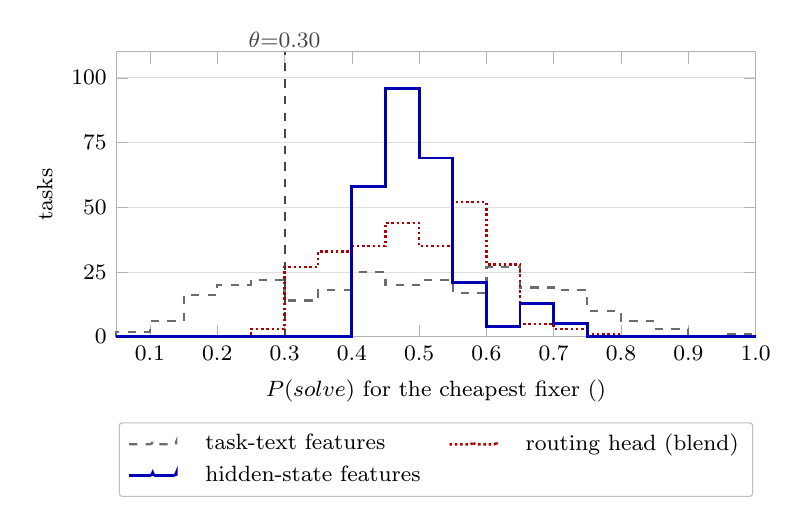
\begin{tikzpicture}
\begin{axis}[
  paperaxis,
  width=0.80\linewidth,
  height=5.2cm,
  xmin=0.05, xmax=1.00,
  ymin=0, ymax=110,
  xtick={0.1,0.2,0.3,0.4,0.5,0.6,0.7,0.8,0.9,1.0},
  xticklabel style={/pgf/number format/fixed,
                    /pgf/number format/fixed zerofill,
                    /pgf/number format/precision=1},
  ytick={0,25,50,75,100},
  xlabel={$P(\text{solve})$ for the cheapest fixer (\fxkimi)},
  ylabel={tasks},
  ymajorgrids=true,
  clip=false,   % lets the \theta tag sit just above the top frame
  legend style={at={(0.5,-0.30)}, anchor=north, legend columns=2,
                column sep=8pt},
  legend cell align=left,
]

% ---- deployed threshold, the ONLY threshold drawn ----------------------
\addplot[gray!55!black, line width=0.7pt, dashed, forget plot]
  coordinates {(0.30,0) (0.30,110)};
\node[font=\footnotesize, text=gray!55!black, anchor=south, inner sep=1.5pt]
  at (axis cs:0.30,110) {$\theta{=}0.30$};

% ---- task-text features (widest, drawn first so it sits behind) --------
\addplot[const plot, cBase!85!black, line width=0.8pt, dashed]
  coordinates {(0.05,0)
    (0.05,2) (0.10,6) (0.15,16) (0.20,20) (0.25,22) (0.30,14)
    (0.35,18) (0.40,25) (0.45,20) (0.50,22) (0.55,17) (0.60,27)
    (0.65,19) (0.70,18) (0.75,10) (0.80,6) (0.85,3) (0.90,0)
    (0.95,1) (1.00,0)};
\addlegendentry{task-text features}

% ---- routing head (uniform average of the two feature heads) -----------
\addplot[const plot, cOpus, line width=0.9pt, densely dotted]
  coordinates {(0.05,0)
    (0.05,0) (0.10,0) (0.15,0) (0.20,0) (0.25,3) (0.30,27)
    (0.35,33) (0.40,35) (0.45,44) (0.50,35) (0.55,52) (0.60,28)
    (0.65,5) (0.70,3) (0.75,1) (0.80,0) (0.85,0) (0.90,0)
    (0.95,0) (1.00,0)};
\addlegendentry{routing head (blend)}

% ---- hidden-state features (the concentrated one, drawn last, on top) --
\addplot[const plot, cSys, line width=1.0pt]
  coordinates {(0.05,0)
    (0.05,0) (0.10,0) (0.15,0) (0.20,0) (0.25,0) (0.30,0)
    (0.35,0) (0.40,58) (0.45,96) (0.50,69) (0.55,21) (0.60,4)
    (0.65,13) (0.70,5) (0.75,0) (0.80,0) (0.85,0) (0.90,0)
    (0.95,0) (1.00,0)};
\addlegendentry{hidden-state features}

\end{axis}
\end{tikzpicture}
